\documentclass[12pt,a4paper]{article}

% ── packages ───────────────────────────────────────────────────────────────
\usepackage[utf8]{inputenc}
\usepackage[T1]{fontenc}
\usepackage[english]{babel}
\usepackage{graphicx}
\usepackage{booktabs}
\usepackage{amsmath}
\usepackage{hyperref}
\usepackage{geometry}
\usepackage{caption}
\usepackage{float}

\geometry{margin=2.5cm}

\title{Custom-WikiCS Graph Analysis -- Part 3\\[4pt]
\large Advanced Analytics: Cleaned Graph, Component Distributions \& Semantic Homogeneity}
\author{}
\date{\today}

\begin{document}
\maketitle

% ═══════════════════════════════════════════════════════════════════════════
\section{Introduction}
% ═══════════════════════════════════════════════════════════════════════════

This third report extends the structural analysis of the Custom-WikiCS graph by introducing advanced analytical techniques. Following feedback from the initial phases, the analysis now focus on a "cleaned" version of the graph where isolated nodes have been removed to ensure that the metrics reflect the interconnected core of the network.

The analyses covered in this phase include:
\begin{enumerate}
    \item Graph pre-processing: Removal of degree-0 isolated nodes.
    \item Detailed component size distribution analysis for weakly and strongly connected components.
    \item Re-calculation of centrality measures (Degree, Betweenness, Closeness, and PageRank) on the cleaned graph, with the addition of \textbf{Eigenvector Centrality}.
    \item Community homogeneity analysis using cosine similarity of node embeddings to validate the semantic coherence of detected clusters.
    \item Correlation analysis between node degree and neighbor similarity.
\end{enumerate}

% ═══════════════════════════════════════════════════════════════════════════
\section{Data Pre-processing: Isolated Node Removal}
% ═══════════════════════════════════════════════════════════════════════════

To refine the analysis, all isolated nodes (nodes with a total degree of 0) were identified and removed. These nodes represent articles that neither link to nor are linked from any other article in the dataset, thus contributing no structural information to the graph.

\begin{table}[H]
\centering
\caption{Graph statistics before and after cleaning.}
\label{tab:cleaning}
\begin{tabular}{lrrr}
\toprule
\textbf{Metric} & \textbf{Original Graph} & \textbf{Cleaned Graph} & \textbf{Reduction} \\
\midrule
Nodes & 11,701 & 11,367 & 334 (2.85\%) \\
Edges & 291,039 & 291,039 & 0 (0.00\%) \\
\bottomrule
\end{tabular}
\end{table}

The removal of \textbf{334 isolated nodes} results in a more robust dataset of 11,367 nodes. While the edge count remains identical, the density and average connectivity metrics are slightly increased, providing a clearer picture of the active network core. All subsequent calculations in this report are performed on this cleaned graph.

% ═══════════════════════════════════════════════════════════════════════════
\section{Component Size Distributions}
% ═══════════════════════════════════════════════════════════════════════════

While the previous report identified the giant components, we now examine the full distribution of component sizes. In directed graphs, the distinction between Weakly Connected Components (WCC) and Strongly Connected Components (SCC) is vital for understanding reachability.

\begin{figure}[H]
    \centering
    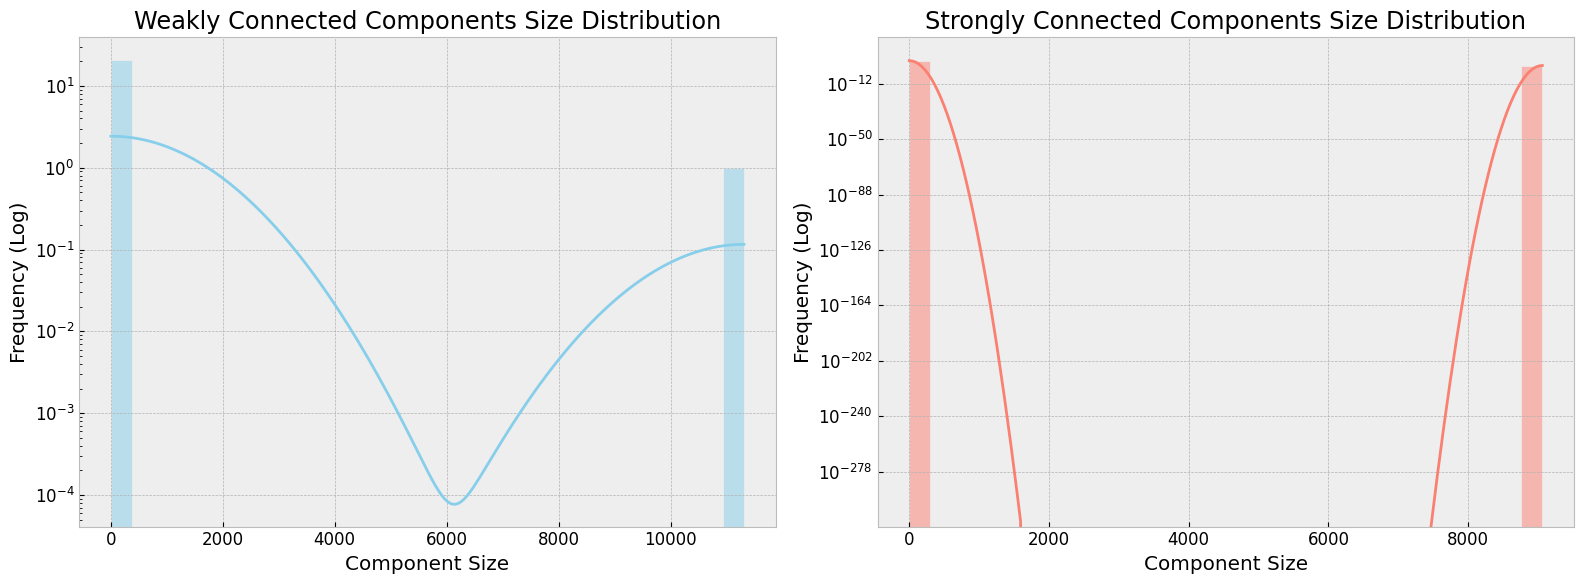
\includegraphics[width=\textwidth]{img-3/component-size-distribution.png}
    \caption{Component size distributions (Log scale): Weakly Connected (left) and Strongly Connected (right).}
    \label{fig:components}
\end{figure}

As shown in Figure~\ref{fig:components}, both distributions exhibit an extreme "winner-takes-all" pattern. For WCCs, the vast majority of nodes are absorbed into a single giant component, with a few tiny peripheral components consisting of just 1 or 2 nodes. The SCC distribution is slightly more fragmented, reflecting the "bow-tie" structure typical of the World Wide Web, where a large core exists alongside smaller in-components and out-components that are not mutually reachable.

% ═══════════════════════════════════════════════════════════════════════════
\section{Centrality Measures Re-evaluation}
% ═══════════════════════════════════════════════════════════════════════════

The centrality measures have been recalculated for the 11,367-node cleaned graph. Additionally, \textbf{Eigenvector Centrality} has been added to measure node influence based on the quality of their connections.

\begin{table}[H]
\centering
\caption{Centrality statistics for the cleaned graph.}
\label{tab:centrality_new}
\begin{tabular}{lrrrr}
\toprule
\textbf{Metric} & \textbf{Min} & \textbf{Max} & \textbf{Mean} & \textbf{Std} \\
\midrule
Degree Centrality & 0.000088 & 0.305648 & 0.004505 & 0.007880 \\
Betweenness Centrality & 0.000000 & 0.215722 & 0.000176 & 0.002481 \\
Closeness Centrality & 0.000000 & 0.550493 & 0.333407 & 0.045880 \\
PageRank & 0.000013 & 0.010007 & 0.000088 & 0.000209 \\
Eigenvector Centrality & 0.000000 & 0.211245 & 0.004355 & 0.008307 \\
\bottomrule
\end{tabular}
\end{table}

The addition of Eigenvector Centrality reveals nodes that are not just highly connected (Degree) but are connected to other influential nodes. Much like PageRank, it is highly skewed (mean $\approx$ 0.0044, max $\approx$ 0.21), suggesting that influence is concentrated in a small "over-connected" elite of articles. The slight increase in mean metrics across all centralities compared to the previous report is a direct result of the removal of isolated (zero-value) nodes.

% ═══════════════════════════════════════════════════════════════════════════
\section{Community Similarity Analysis}
% ═══════════════════════════════════════════════════════════════════════════

To evaluate whether the structural communities detected by the Louvain algorithm correspond to semantically homogeneous groups, we analyzed the cosine similarity of node embeddings.

\begin{table}[H]
\centering
\caption{Average Cosine Similarity of node embeddings.}
\label{tab:similarity}
\begin{tabular}{lr}
\toprule
\textbf{Category} & \textbf{Average Cosine Similarity} \\
\midrule
Intra-community (Inner links) & \textbf{0.5795} \\
Inter-community (Outer links) & 0.5481 \\
\bottomrule
\end{tabular}
\end{table}

The results support the hypothesis of thematic clustering: nodes within the same community share a higher average similarity (\textbf{0.5795}) than nodes connected across different communities (0.5481). This difference, while subtle, indicates that the Louvain algorithm's structural partitions successfully capture groups of articles with related topical content.

% ═══════════════════════════════════════════════════════════════════════════
\section{Node Degree vs. Semantic Similarity}
% ═══════════════════════════════════════════════════════════════════════════

Finally, we explored whether a node's topological importance (degree) correlates with the semantic similarity of its neighbors. Nodes were binned by degree ranges, and the average neighbor similarity was calculated.

\begin{figure}[H]
    \centering
    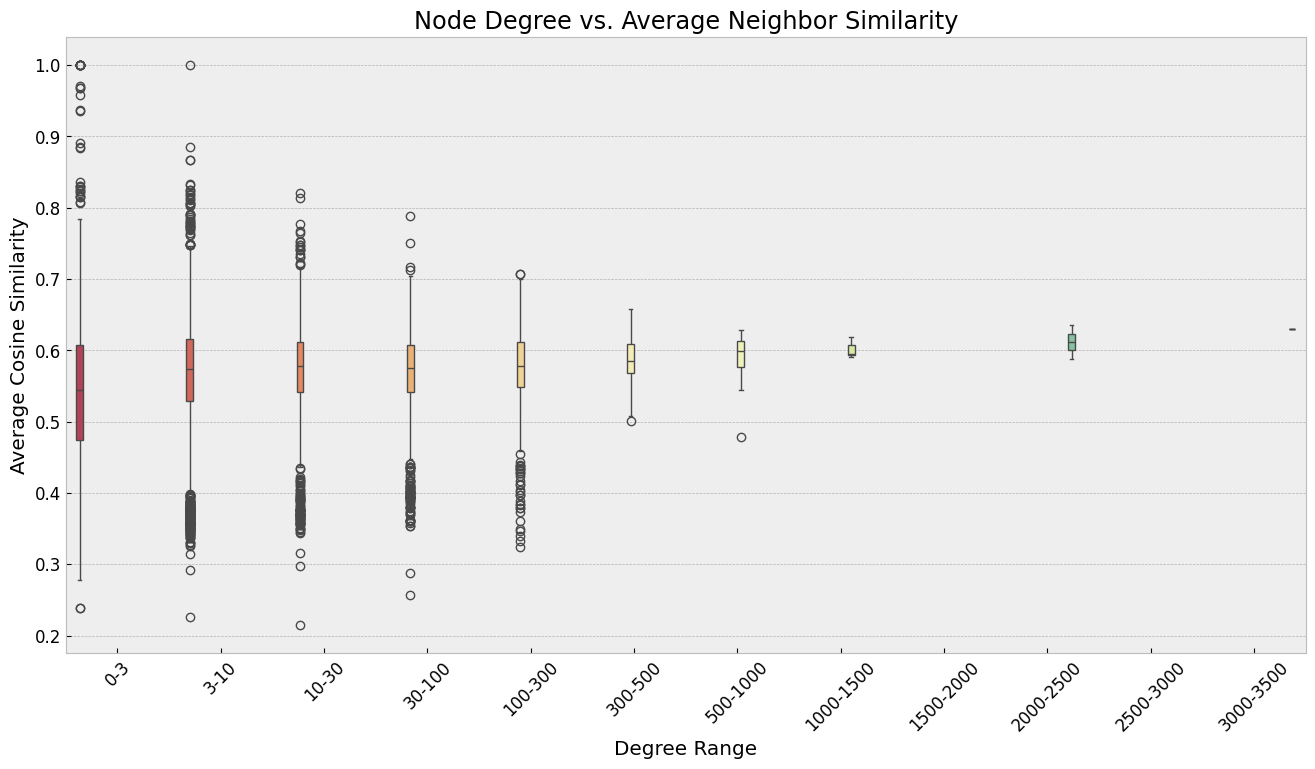
\includegraphics[width=0.85\textwidth]{img-3/node-degree-vs-neighbor-similarity.png}
    \caption{Node degree vs. average neighbor similarity distribution.}
    \label{fig:degree_sim}
\end{figure}

The box plot in Figure~\ref{fig:degree_sim} illustrates that nodes with very high degrees tend to have neighbor similarity distributions that converge towards the global mean, acting as generalist hubs. In contrast, lower-degree nodes often show higher variance in neighbor similarity, with some being part of highly specific, semantically tight-knit niches.

% ═══════════════════════════════════════════════════════════════════════════
\section{Conclusion}
% ═══════════════════════════════════════════════════════════════════════════

Phase 3 of the Custom-WikiCS analysis has demonstrated that:
\begin{itemize}
    \item Removing the 334 isolated nodes provides a cleaner structural baseline for the network.
    \item Eigenvector centrality identifies a distinct tier of influential articles that form the "prestige" core of the Wikipedia category.
    \item There is a clear alignment between topological community structure and semantic embedding similarity, confirming that links on Wikipedia are driven by topical relevance.
    \item The relationship between degree and similarity suggests a hierarchical organization where specialized articles connect to broader hubs.
\end{itemize}

\end{document}
